
%% bare_conf.tex
%% V1.4b
%% 2015/08/26
%% by Michael Shell
%% See:
%% http://www.michaelshell.org/
%% for current contact information.
%%
%% This is a skeleton file demonstrating the use of IEEEtran.cls
%% (requires IEEEtran.cls version 1.8b or later) with an IEEE
%% conference paper.
%%
%% Support sites:
%% http://www.michaelshell.org/tex/ieeetran/
%% http://www.ctan.org/pkg/ieeetran
%% and
%% http://www.ieee.org/

%%*************************************************************************
%% Legal Notice:
%% This code is offered as-is without any warranty either expressed or
%% implied; without even the implied warranty of MERCHANTABILITY or
%% FITNESS FOR A PARTICULAR PURPOSE! 
%% User assumes all risk.
%% In no event shall the IEEE or any contributor to this code be liable for
%% any damages or losses, including, but not limited to, incidental,
%% consequential, or any other damages, resulting from the use or misuse
%% of any information contained here.
%%
%% All comments are the opinions of their respective authors and are not
%% necessarily endorsed by the IEEE.
%%
%% This work is distributed under the LaTeX Project Public License (LPPL)
%% ( http://www.latex-project.org/ ) version 1.3, and may be freely used,
%% distributed and modified. A copy of the LPPL, version 1.3, is included
%% in the base LaTeX documentation of all distributions of LaTeX released
%% 2003/12/01 or later.
%% Retain all contribution notices and credits.
%% ** Modified files should be clearly indicated as such, including  **
%% ** renaming them and changing author support contact information. **
%%*************************************************************************


% *** Authors should verify (and, if needed, correct) their LaTeX system  ***
% *** with the testflow diagnostic prior to trusting their LaTeX platform ***
% *** with production work. The IEEE's font choices and paper sizes can   ***
% *** trigger bugs that do not appear when using other class files.       ***                          ***
% The testflow support page is at:
% http://www.michaelshell.org/tex/testflow/



\documentclass[conference]{IEEEtran}
% Some Computer Society conferences also require the compsoc mode option,
% but others use the standard conference format.
%
% If IEEEtran.cls has not been installed into the LaTeX system files,
% manually specify the path to it like:
% \documentclass[conference]{../sty/IEEEtran}





% Some very useful LaTeX packages include:
% (uncomment the ones you want to load)


% *** MISC UTILITY PACKAGES ***
%
%\usepackage{ifpdf}
% Heiko Oberdiek's ifpdf.sty is very useful if you need conditional
% compilation based on whether the output is pdf or dvi.
% usage:
% \ifpdf
%   % pdf code
% \else
%   % dvi code
% \fi
% The latest version of ifpdf.sty can be obtained from:
% http://www.ctan.org/pkg/ifpdf
% Also, note that IEEEtran.cls V1.7 and later provides a builtin
% \ifCLASSINFOpdf conditional that works the same way.
% When switching from latex to pdflatex and vice-versa, the compiler may
% have to be run twice to clear warning/error messages.






% *** CITATION PACKAGES ***
%
%\usepackage{cite}
% cite.sty was written by Donald Arseneau
% V1.6 and later of IEEEtran pre-defines the format of the cite.sty package
% \cite{} output to follow that of the IEEE. Loading the cite package will
% result in citation numbers being automatically sorted and properly
% "compressed/ranged". e.g., [1], [9], [2], [7], [5], [6] without using
% cite.sty will become [1], [2], [5]--[7], [9] using cite.sty. cite.sty's
% \cite will automatically add leading space, if needed. Use cite.sty's
% noadjust option (cite.sty V3.8 and later) if you want to turn this off
% such as if a citation ever needs to be enclosed in parenthesis.
% cite.sty is already installed on most LaTeX systems. Be sure and use
% version 5.0 (2009-03-20) and later if using hyperref.sty.
% The latest version can be obtained at:
% http://www.ctan.org/pkg/cite
% The documentation is contained in the cite.sty file itself.






% *** GRAPHICS RELATED PACKAGES ***
%
\ifCLASSINFOpdf
  % \usepackage[pdftex]{graphicx}
  % declare the path(s) where your graphic files are
  % \graphicspath{{../pdf/}{../jpeg/}}
  % and their extensions so you won't have to specify these with
  % every instance of \includegraphics
  % \DeclareGraphicsExtensions{.pdf,.jpeg,.png}
\else
  % or other class option (dvipsone, dvipdf, if not using dvips). graphicx
  % will default to the driver specified in the system graphics.cfg if no
  % driver is specified.
  % \usepackage[dvips]{graphicx}
  % declare the path(s) where your graphic files are
  % \graphicspath{{../eps/}}
  % and their extensions so you won't have to specify these with
  % every instance of \includegraphics
  % \DeclareGraphicsExtensions{.eps}
\fi
% graphicx was written by David Carlisle and Sebastian Rahtz. It is
% required if you want graphics, photos, etc. graphicx.sty is already
% installed on most LaTeX systems. The latest version and documentation
% can be obtained at: 
% http://www.ctan.org/pkg/graphicx
% Another good source of documentation is "Using Imported Graphics in
% LaTeX2e" by Keith Reckdahl which can be found at:
% http://www.ctan.org/pkg/epslatex
%
% latex, and pdflatex in dvi mode, support graphics in encapsulated
% postscript (.eps) format. pdflatex in pdf mode supports graphics
% in .pdf, .jpeg, .png and .mps (metapost) formats. Users should ensure
% that all non-photo figures use a vector format (.eps, .pdf, .mps) and
% not a bitmapped formats (.jpeg, .png). The IEEE frowns on bitmapped formats
% which can result in "jaggedy"/blurry rendering of lines and letters as
% well as large increases in file sizes.
%
% You can find documentation about the pdfTeX application at:
% http://www.tug.org/applications/pdftex





% *** MATH PACKAGES ***
%
%\usepackage{amsmath}
% A popular package from the American Mathematical Society that provides
% many useful and powerful commands for dealing with mathematics.
%
% Note that the amsmath package sets \interdisplaylinepenalty to 10000
% thus preventing page breaks from occurring within multiline equations. Use:
%\interdisplaylinepenalty=2500
% after loading amsmath to restore such page breaks as IEEEtran.cls normally
% does. amsmath.sty is already installed on most LaTeX systems. The latest
% version and documentation can be obtained at:
% http://www.ctan.org/pkg/amsmath





% *** SPECIALIZED LIST PACKAGES ***
%
%\usepackage{algorithmic}
% algorithmic.sty was written by Peter Williams and Rogerio Brito.
% This package provides an algorithmic environment fo describing algorithms.
% You can use the algorithmic environment in-text or within a figure
% environment to provide for a floating algorithm. Do NOT use the algorithm
% floating environment provided by algorithm.sty (by the same authors) or
% algorithm2e.sty (by Christophe Fiorio) as the IEEE does not use dedicated
% algorithm float types and packages that provide these will not provide
% correct IEEE style captions. The latest version and documentation of
% algorithmic.sty can be obtained at:
% http://www.ctan.org/pkg/algorithms
% Also of interest may be the (relatively newer and more customizable)
% algorithmicx.sty package by Szasz Janos:
% http://www.ctan.org/pkg/algorithmicx




% *** ALIGNMENT PACKAGES ***
%
%\usepackage{array}
% Frank Mittelbach's and David Carlisle's array.sty patches and improves
% the standard LaTeX2e array and tabular environments to provide better
% appearance and additional user controls. As the default LaTeX2e table
% generation code is lacking to the point of almost being broken with
% respect to the quality of the end results, all users are strongly
% advised to use an enhanced (at the very least that provided by array.sty)
% set of table tools. array.sty is already installed on most systems. The
% latest version and documentation can be obtained at:
% http://www.ctan.org/pkg/array


% IEEEtran contains the IEEEeqnarray family of commands that can be used to
% generate multiline equations as well as matrices, tables, etc., of high
% quality.




% *** SUBFIGURE PACKAGES ***
%\ifCLASSOPTIONcompsoc
%  \usepackage[caption=false,font=normalsize,labelfont=sf,textfont=sf]{subfig}
%\else
%  \usepackage[caption=false,font=footnotesize]{subfig}
%\fi
% subfig.sty, written by Steven Douglas Cochran, is the modern replacement
% for subfigure.sty, the latter of which is no longer maintained and is
% incompatible with some LaTeX packages including fixltx2e. However,
% subfig.sty requires and automatically loads Axel Sommerfeldt's caption.sty
% which will override IEEEtran.cls' handling of captions and this will result
% in non-IEEE style figure/table captions. To prevent this problem, be sure
% and invoke subfig.sty's "caption=false" package option (available since
% subfig.sty version 1.3, 2005/06/28) as this is will preserve IEEEtran.cls
% handling of captions.
% Note that the Computer Society format requires a larger sans serif font
% than the serif footnote size font used in traditional IEEE formatting
% and thus the need to invoke different subfig.sty package options depending
% on whether compsoc mode has been enabled.
%
% The latest version and documentation of subfig.sty can be obtained at:
% http://www.ctan.org/pkg/subfig




% *** FLOAT PACKAGES ***
%
%\usepackage{fixltx2e}
% fixltx2e, the successor to the earlier fix2col.sty, was written by
% Frank Mittelbach and David Carlisle. This package corrects a few problems
% in the LaTeX2e kernel, the most notable of which is that in current
% LaTeX2e releases, the ordering of single and double column floats is not
% guaranteed to be preserved. Thus, an unpatched LaTeX2e can allow a
% single column figure to be placed prior to an earlier double column
% figure.
% Be aware that LaTeX2e kernels dated 2015 and later have fixltx2e.sty's
% corrections already built into the system in which case a warning will
% be issued if an attempt is made to load fixltx2e.sty as it is no longer
% needed.
% The latest version and documentation can be found at:
% http://www.ctan.org/pkg/fixltx2e


%\usepackage{stfloats}
% stfloats.sty was written by Sigitas Tolusis. This package gives LaTeX2e
% the ability to do double column floats at the bottom of the page as well
% as the top. (e.g., "\begin{figure*}[!b]" is not normally possible in
% LaTeX2e). It also provides a command:
%\fnbelowfloat
% to enable the placement of footnotes below bottom floats (the standard
% LaTeX2e kernel puts them above bottom floats). This is an invasive package
% which rewrites many portions of the LaTeX2e float routines. It may not work
% with other packages that modify the LaTeX2e float routines. The latest
% version and documentation can be obtained at:
% http://www.ctan.org/pkg/stfloats
% Do not use the stfloats baselinefloat ability as the IEEE does not allow
% \baselineskip to stretch. Authors submitting work to the IEEE should note
% that the IEEE rarely uses double column equations and that authors should try
% to avoid such use. Do not be tempted to use the cuted.sty or midfloat.sty
% packages (also by Sigitas Tolusis) as the IEEE does not format its papers in
% such ways.
% Do not attempt to use stfloats with fixltx2e as they are incompatible.
% Instead, use Morten Hogholm'a dblfloatfix which combines the features
% of both fixltx2e and stfloats:
%
% \usepackage{dblfloatfix}
% The latest version can be found at:
% http://www.ctan.org/pkg/dblfloatfix




% *** PDF, URL AND HYPERLINK PACKAGES ***
%
%\usepackage{url}
% url.sty was written by Donald Arseneau. It provides better support for
% handling and breaking URLs. url.sty is already installed on most LaTeX
% systems. The latest version and documentation can be obtained at:
% http://www.ctan.org/pkg/url
% Basically, \url{my_url_here}.




% *** Do not adjust lengths that control margins, column widths, etc. ***
% *** Do not use packages that alter fonts (such as pslatex).         ***
% There should be no need to do such things with IEEEtran.cls V1.6 and later.
% (Unless specifically asked to do so by the journal or conference you plan
% to submit to, of course. )


% correct bad hyphenation here
\hyphenation{op-tical net-works semi-conduc-tor}


%\usepackage{xspace}
\usepackage{proof}
\usepackage{graphicx}
\usepackage{pdfpages}
\usepackage{amsmath}
\usepackage{amsthm}
\usepackage{amscd}
\usepackage{amssymb}
\usepackage{float}
\usepackage{epsfig}
\usepackage{xcolor}
\usepackage{color}
%\usepackage{subfig}
\usepackage{subcaption}
\usepackage{filecontents}
\usepackage{moresize}

%\usepackage[sort&compress]{natbib}

% use latin modern font
\usepackage[T1]{fontenc}
%\usepackage{lmodern}
\usepackage[kerning,spacing]{microtype}
 
%\floatstyle{boxed}
%\restylefloat{figure}


\newcommand{\TODO}[1]{[\textsl{#1}]}
%\newcommand{\comment}[1]{[\textsl{#1}]}
\newcommand{\hide}[1]{} 
\newcommand{\C}[1]{\lstinline!#1!}
\newcommand {\spc}{\hspace{3pt}}
\newcommand{\spmd}{\textsc{spmd}}
\newcommand{\cegis}{\textsc{cegis}}
\newcommand{\Sk}{\textsc{Sketch}}
\newcommand{\Lang}{\textsc{Imp}~}
\newcommand{\LangSk}{\textsc{ImpSynt}~}
\hyphenation{spmd cegis Sketch MSL Jacobi}

\newcommand{\constraintenv}{\Sigma}
\newcommand{\cfun}{\gamma}
%%% Inference rule things.
\newcommand{\integ}{\mbox{\texttt{int}}}
%%%%%%%%%%%%%%%%%%%%%%%%%%%%%%%%%%%%%%%%%%%
% Macros for the semantics
%%%%%%%%%%%%%%%%%%%%%%%%%%%%%%%%%%%%%%%%%%%

\newcommand{\valEnv}{\Sigma}
\newcommand{\typeEnv}{\Gamma}
\newcommand{\cdeclEnv}{\Pi}
\newcommand{\cEnv}{\Lambda}

%%%%%%%%%%%%%%%%%%%%%%%%%%%%%%%%%%%%%%%%%%%
%%%%%%%%%%%%%%%%%%%%%%%%%%%%%%%%%%%%%%%%%%

\newcommand{\etal}{\textit{et al.}\@\xspace}
\newcommand{\eg}{\textit{e.g.}\@\xspace}
\newcommand{\ie}{\textit{i.e.}\@\xspace}

% References
%
%\newtheorem{thm}{Theorem}
\newtheorem{lem}{Lemma}
\newtheorem{prop}{Property}

\newcommand{\thmlabel}[1]{\label{thm:#1}}
\newcommand{\thmref}[1]{Theorem~\ref{thm:#1}}
\newcommand{\lemlabel}[1]{\label{lem:#1}}
\newcommand{\lemref}[1]{Lemma~\ref{lem:#1}}

\newcommand{\corlabel}[1]{\label{cor:#1}}
\newcommand{\corref}[1]{Corollary~\ref{cor:#1}}

\newcommand{\proplabel}[1]{\label{prop:#1}}
\newcommand{\propref}[1]{Proposition~\ref{prop:#1}}
\newcommand{\deflabel}[1]{\label{def:#1}}
\newcommand{\defref}[1]{Definition~\ref{def:#1}}
\newcommand{\exlabel}[1]{\label{ex:#1}}
\newcommand{\exref}[1]{Example~\ref{ex:#1}}
\newcommand{\problabel}[1]{\label{prob:#1}}
\newcommand{\probref}[1]{Problem~\ref{prob:#1}}
\newcommand{\obslabel}[1]{\label{obs:#1}}
\newcommand{\obsref}[1]{Observation~\ref{obs:#1}}
\newcommand{\alglabel}[1]{\label{alg:#1}}
\newcommand{\algref}[1]{Algorithm~\ref{alg:#1}}
%
\newcommand{\applabel}[1]{\label{app:#1}}
\newcommand{\appref}[1]{Appendix~\ref{app:#1}}
\newcommand{\seclabel}[1]{\label{sec:#1}}
\newcommand{\shortsecref}[1]{\S\ref{sec:#1}}
\newcommand{\longsecref}[1]{Section~\ref{sec:#1}}
%
\newcommand{\tablabel}[1]{\label{tab:#1}}
\newcommand{\tabref}[1]{Table~\ref{tab:#1}}
\newcommand{\figlabel}[1]{\label{fig:#1}}
\newcommand{\longfigref}[1]{Figure~\ref{fig:#1}}
\newcommand{\shortfigref}[1]{Fig.~\ref{fig:#1}}
\newcommand{\eqqlabel}[1]{\label{eq:#1}}
\newcommand{\shorteqqref}[1]{\eqref{eq:#1}}
\newcommand{\mediumeqqref}[1]{Eq.~\eqref{eq:#1}}
\newcommand{\longeqqref}[1]{Equation~\eqref{eq:#1}}

% Determine type of references for particular document.
%
\newcommand{\secref}{\longsecref}
\newcommand{\figref}{\longfigref}
\newcommand{\eqqref}{\longeqqref}

% Numbering layout
%
\numberwithin{equation}{section}
%\newtheorem{definition}{Definition}
%\newtheorem{corollary}{Corollary}
\newtheorem{hypothesis}{Hypothesis}
\newtheorem{algo}{Algorithm}
\newtheorem{Equation}{Equation}
%\newtheorem{theorem}{Theorem}


                     %%% Commands for formatting code %%%

\newcommand{\while}{\textbf{\texttt{while}}}
\newcommand{\init}{\textbf{\texttt{init}}}
\newcommand{\decreases}{\textbf{\texttt{decreases}}}

% \token -- used for a literal code token
% \nterm -- used for a grammar non-terminal
% Example:  Every \nterm{AssertStmt} begins with the \token{assert} keyword.
\newcommand{\token}[1]{\code{#1}}
\newcommand{\formatnt}[1]{{\sl#1}}  % This _must_ be {\sl#1}, not \textsl{#1}
\newcommand{\nterm}[1]{\index{#1@\formatnt{#1}}\formatnt{#1}}

% syntax -- environment for specifiying syntax
\newenvironment{syntax}
 {\par\begin{tabular}{rcl}}
 {\end{tabular}\vspace{2ex}}

% \lexrule -- used to define a lexical regexp rule within a syntax environment
% Example:  \lexrule{IntegerLiteral}{[0-9]+}
\newcommand{\lexrule}[2]
 {\index{#1@\formatnt{#1}|defpage}\formatnt{#1} &
  $=$ & $\langle${\tt#2}$\rangle$ \\}

% \grammar -- used to define a grammar non-terminal within a syntax environment
% \grammaralt -- used for alternate definitions within a syntax environment
% Example:  \grammar{Expr}{\nterm{Expr} \token{+} \nterm{Expr}}
%           \grammaralt{\token{(} \nterm{Expr} \token{)}}
\newcommand{\grammar}[2]
 {\index{#1@\formatnt{#1}|defpage}\formatnt{#1} & $=$ & {#2} \\}
\newcommand{\grammaralt}[1]{& $|$ & {#1} \\}
\newcommand{\grammarelt}[2]
 {\index{#1@\formatnt{#1}|defpage}\formatnt{#1} & $\in$ & {#2} \\}

\newcommand{\galt}{\mbox{\hspace{0.7em}\ensuremath{|}\hspace{1em}}}

%%% Commands for inserting special characters %%%

% \bs -- used to create a monospace backslash
\newcommand{\bs}{{\tt\char"5C}}

% \us -- used to create a monospace underscore (works better than {\tt\_})
\newcommand{\us}{{\tt\char"5F}}


\usepackage[T1]{fontenc}
%\usepackage[scaled=0.85]{luximono}


\definecolor{dkgreen}{rgb}{0,0.3,0}
\definecolor{gray}{rgb}{0.5,0.5,0.5}
\definecolor{mauve}{rgb}{0.58,0,0.82}
\definecolor{light-gray}{gray}{0.80}

\usepackage{listings}
\lstdefinelanguage{spmd}{
  morekeywords = {
       loc, bit, bool, true, false
     , implements, harness
     , null
     , assert, assume
     , else
     , find, fix, fold, for, forall, function
     , generator, gen
     , if, while, int, float, bool, string
     , loop, simple, cond, val
     , fork, join
     , nil, null, none, new, malloc
     , option, or
     , ref, return
     , spmdfork, nprocs, spmdtransfer
     , void
     , concrete, sym
     , requires, ensures
     , invariant, decreases 
     , conj, exp
     , init, stmt},
  literate=
    {-}{--}1,
  morecomment=[l]{//}
}
\lstset{
  language=spmd,
  columns=flexible,
% basicstyle=\fontfamily{lmss}\selectfont\tiny,
  basicstyle=\fontfamily{lmss}\fontsize{7.5pt}{5pt}\selectfont,
  numbers=none,
  numbersep=3pt,
  numberstyle=\tiny,
  stepnumber=1,
  tabsize=2,      
  breaklines=false,  
  breakatwhitespace=true,
  mathescape=true,
  commentstyle=\color{cyan},
  escapechar=^,
%  escapeinside={\%*}{*)}   
}




\renewcommand{\scriptsize}{\fontsize{8.5}{9}\selectfont}
\makeatletter
\lst@AddToHook{TextStyle}{\let\lst@basicstyle\scriptsize\fontfamily{lmss}\selectfont}
\makeatother

\usepackage{url}

\newcommand{\pr}[1]{\left(#1\right)}
\renewcommand{\t}[1]{\text{#1}}
\renewcommand{\b}[1]{\t{\lstinline{#1}}}
\newcommand{\msc}[1]{\ensuremath{\text{{\texttt{#1}}}}}
%\renewcommand{\hss}{\hspace{\stretch{1}}}
\renewcommand{\vss}{\vspace{10pt}}
\newcommand{\sem}[1]{[\![#1]\!]}
\newcommand{\esem}[1]{\mathcal{E}[\![#1]\!]}
\newcommand{\tsem}[1]{\mathcal{T}[\![#1]\!]}
\newcommand{\lam}[2]{\ensuremath{\lambda #1 .\hspace{0.01em} #2}}
\newcommand{\allq}[2]{\ensuremath{\forall #1 .\hspace{0.01em} #2}}
\newcommand{\dbr}[2]{\ensuremath{\{\hspace{-0.2em}| \,#1\,|\,#2\, |\hspace{-0.2em}\}}}
\newcommand{\secsp}{\vspace*{20pt}}

\newcommand{\csubtype}{<:_c}
\newcommand{\fsubtype}{<:_f}
\newcommand{\lub}{\sqcup}
\newcommand{\biglub}{\bigsqcup}
\newcommand{\guard}{\mathcal{G}}

\newcommand{\tenv}{\Gamma}
\newcommand{\denv}{\Delta}
\newcommand{\cenv}{\Sigma}

\newcommand{\stack}[2]{\genfrac{}{}{0pt}{0}{#1}{#2}}

\newcommand{\ors}{\ensuremath{\ |\ \ }}
\newcommand{\deriv}[5]{#1 \vdash \langle #2, #3 \rangle \rightarrow \langle #4, #5 \rangle}
\newcommand{\derivstar}[5]{#1 \vdash \langle #2, #3 \rangle \rightarrow^* \langle #4, #5 \rangle}
\newcommand{\tcrule}[3]{#1 \vdash^c #2 : #3 }
\newcommand{\tdrule}[3]{#1 \vdash #2 : #3}

\newcommand{\nrec}{\stackrel{nr}{\rightarrow}}

% Variables used in symantics and proofs.
\newcommand{\cprim}{c}
\newcommand{\constraint}{\gamma}
\newcommand{\model}{\msc{Model}}
\newcommand{\symbolic}{\sigma}
\newcommand{\store}{\sigma}
\newcommand{\irreducible}{\upsilon}
\newcommand{\levels}{\mathcal{L}}
\newcommand{\lorder}{\sqsubseteq_\levels}
\newcommand{\unsat}{\msc{Unsat}}
\newcommand{\translatesto}{\hookrightarrow}

% For properties...
\newcommand{\spair}[3]{\langle #1 | #2 \rangle_#3}
\newcommand{\cproj}[3]{[#1]_{#2, #3}}

\newcommand{\basetype}{\beta}
\newcommand{\typair}[2]{\langle #1, #2 \rangle}


% Comments
\newcommand{\comment}[3][\color{red}]{{#1{[{#2}: {#3}]}}}
\newcommand{\asolar}[1]{\comment[\color{red}]{ASL}{#1}}
%\newcommand{\xkqiu}[1]{\comment[\color{cyan}]{XKQ}{#1}}
\newcommand{\xkqiu}[1]{}

% Uninterpreted function
\newcommand{\oracle}{\textit{Orcl}}

\renewcommand{\floatpagefraction}{.9}%


\def\Cpp{C{}\texttt{++}~}





















\usepackage{rotating}

%\lstset{language=C}
\lstset{columns=fullflexible, basicstyle=\ttfamily}
\usepackage{enumitem}
%\usepackage[breaklinks]{hyperref}

%%\hypersetup{pdfborder={0 0 100}}
%%\usepackage[hyphens]{url}

\usepackage{algorithm2e}
\usepackage{gastex}
\usepackage{multirow}

\newcommand{\lstc}[1]{\text{\lstinline{#1}}}

%\newtheorem{theorem}{Theorem}[section]
%\newtheorem{lemma}[theorem]{Lemma}
%\newtheorem{proposition}[theorem]{Proposition}
%\newtheorem{corollary}[theorem]{Corollary}
%\newtheorem{definition}[theorem]{Definition}
%\newtheorem{example}[theorem]{Example}

\newcommand{\T}{T_\textit{VCC}}

\newcommand{\code}[1]{\textsf{#1}}

\newcommand{\conf}[1]{}
\newcommand{\techrep}[1]{#1}

\newcommand{\Mona}{\textsc{Mona}\xspace}

%\newcommand{\Dryad}{\textsc{Dryad}$_\textrm{sep}$\xspace}
%\newenvironment{proof}[1][Proof]{\begin{trivlist}
%\item[\hskip \labelsep {\bfseries #1}]}{\end{trivlist}}
\newcommand{\dryadtree}{\textsc{Dryad}$_\textrm{tree}$\xspace}
\newcommand{\Dryaddec}{\textsc{Dryad}$^\textrm{dec}_\textrm{tree}$\xspace}

%\newcommand{\head}{{\tt head}\xspace}
%\newcommand{\tail}{{\tt tail}\xspace}
%\newcommand{\rroot}{{\tt root}\xspace}
%\newcommand{\nnext}{{\tt next}\xspace}
%\newcommand{\pprev}{{\tt prev}\xspace}
%\newcommand{\loglisthead}{{\tt log\_listhead}\xspace}
%\newcommand{\chname}{{\tt chname}\xspace}
%\newcommand{\filename}{{\tt filename}\xspace}
%\newcommand{\data}{{\tt data}\xspace}

\newcommand{\error}{{\textit{error}}\xspace}
\newcommand{\ffalse}{{{\tt false}}\xspace}
\newcommand{\ttrue}{{{\tt true}}\xspace}
\newcommand{\f}{{\textit{f}}\xspace}
\newcommand{\g}{{\textit{g}}\xspace}

\newcommand{\Dryadorig}{{\sc Dryad}\xspace}
\newcommand{\Dryad}{{\sc Dryad}$^\textrm{FO}$\xspace}

\newcommand{\head}{{\tt head}\xspace}
\newcommand{\tail}{{\tt tail}\xspace}
\newcommand{\rroot}{{\tt root}\xspace}
\newcommand{\nnext}{{\tt next}\xspace}
\newcommand{\pprev}{{\tt prev}\xspace}
\newcommand{\loglisthead}{{\tt log\_listhead}\xspace}
\newcommand{\chname}{{\tt chname}\xspace}
%\newcommand{\filename}{{\tt filename}\xspace}
\newcommand{\data}{{\tt data}\xspace}
\newcommand{\stmt}{{\tt Stmt}\xspace}
\newcommand{\strfields}{{F}\xspace}

\newcommand{\st}{{\textit st}}
\newcommand{\equal}{{\textit{equal}}}
\newcommand{\dt}{{\textit{dt}}}
\newcommand{\Nadapt}{{\textit Nadapt}}


\newcommand{\adapt}{{\textit{adapt}}}
\newcommand{\Active}{{\textit{active}}}
\newcommand{\nilnode}{{\textit{xnil}}}
\newcommand{\nil}{{\textit{nil}}}
\newcommand{\niltt}{\texttt{nil}\xspace}
\newcommand{\Assume}{{\texttt{assume}}}

\newcommand{\h}{{\textit{h}}}
\newcommand{\rr}{{\textit{r}}}
\newcommand{\p}{{\textit{p}}}
\newcommand{\q}{{\textit{q}}}
\newcommand{\z}{{\textit{z}}}
\newcommand{\x}{{\textit{x}}}
\newcommand{\y}{{\textit{y}}}
\newcommand{\ex}{{\textit{ex}}}
\newcommand{\new}{{\textit{new}}}
\newcommand{\newnode}{{\textit{new}}}
\newcommand{\free}{{\textit{free}}}
\newcommand{\nilvar}{{\textit{nil}}}
\newcommand{\undefined}{{\textit{ndef}}}
\newcommand{\Var}{{\textit{Var}}}

\renewcommand{\implies}{\Rightarrow}

\newcommand{\tuple}[1]{\langle #1 \rangle}
%\newcommand{\ignore}[1]{}
\newcommand{\pc}{\textit{pc}}
\newcommand{\Goal}{\mbox{\textit{Target}}}
\newcommand{\Loc}{\textit{Local}}
\newcommand{\G}{\textit{Global}}
\newcommand{\PC}{\textit{PC}}
\newcommand{\Params}{\mbox{\textit{Par}}}
\newcommand{\atomic}{\mbox{\textit{atom}}}

\newcommand{\calP}{{\cal P}}
\newcommand{\eager}{\mbox{Eager}}
%\newcommand{\qed}{\hfill \mbox{\raggedright \rule{.07in}{.1in}}}

\newcommand{\Strand}{{\sc Strand}\xspace}
\newcommand{\Stranddecsem}{{\sc Strand}\ensuremath{_\textit{dec}^\textit{sem}}\xspace}
\newcommand{\Stranddec}{{\sc Strand}\ensuremath{_\textit{dec}^\textit{syn}}\xspace}
\newcommand{\Stranddecbold}{{\bfseries\scshape Strand}\ensuremath{_\textit{\bfseries dec}^\textit{\bfseries sem}}}
\newcommand{\Stranddecsyn}{{\sc Strand}\ensuremath{_\textit{dec}^\textit{syn}}\xspace}
\newcommand{\Stranddecsynbold}{{\scshape \bfseries Strand}\ensuremath{_\textit{\bfseries dec}}}
\newcommand{\Stranddectree}{{\sc Strand}\ensuremath{_\textit{dec}^{\textit{tree}}}}
\newcommand{\ValidSubmodel}{\textit{ValidSubModel}}
\newcommand{\Subtree}{\textit{Subtree}}
\newcommand{\Graph}{\textit{Graph}}

\newcommand{\SH}{\textit{SH}}
\newcommand{\CH}{\textit{CH}}
\newcommand{\df}{\textit{df}}
\newcommand{\edf}{f}
\newcommand{\DF}{\textit{DF}}
\newcommand{\pv}{\textit{pv}}
\newcommand{\PV}{\textit{PV}}
\newcommand{\pre}{\textit{pre}}
\newcommand{\post}{\textit{post}}
\newcommand{\Pre}{\textit{Pre}}
\newcommand{\Post}{\textit{Post}}
\newcommand{\trans}{\textit{trans}}
\newcommand{\inv}{\textit{inv}}
\newcommand{\syn}{\textit{syn}}
\newcommand{\ite}{\textsf{ite}}
\newcommand{\dir}{\textit{dir}}
\newcommand{\edir}{d}
\newcommand{\Dir}{\textit{PF}}
\newcommand{\FP}{\textit{F\!P}}
\newcommand{\old}{\textit{old}}
\newcommand{\Def}{\textit{Def}}
\newcommand{\base}{\textit{base}}
\newcommand{\ind}{\textit{ind}}
\newcommand{\aexpr}{\textit{aexpr}}
\newcommand{\bexpr}{\textit{bexpr}}
\newcommand{\TS}{\textit{T\!S}}
%\newcommand{\ts}{\textit{ts}}
\newcommand{\Cc}{{C^c}}
\newcommand{\ccnil}{{c_{\textit nil}^c}}
\newcommand{\dirc}{{\textit{dir}^c}}
\newcommand{\dfc}{{\textit{df}^c}}
\newcommand{\pvc}{{\textit{pv}^c}}

\newcommand{\expand}{\textit{expand}}
\newcommand{\funrestrict}[2]{{#1} \mid_{#2}}
\newcommand{\funsubst}[3]{{#1}[{#2} \leftarrow {#3}]}
\newcommand{\formsubst}[3]{{#1}[{#2} / {#3}]}


\newcommand{\vecx}{\vec{x}}
\newcommand{\vecc}{\vec{c}}

\newcommand{\key}{\textit{key}}
\newcommand{\keys}{\textit{keys}}
\newcommand{\bst}{\textit{bst}}
\newcommand{\LEFT}{\textit{left}}
\newcommand{\RIGHT}{\textit{right}}

\newcommand{\pf}{\textit{pf}}
\newcommand{\PF}{\textit{PF}}
\newcommand{\vect}[1]{\,\overrightarrow{\!\!#1}}
\newcommand{\ret}{\textit{ret}}
\newcommand{\precall}{\textit{pre\_call}}
\newcommand{\postcall}{\textit{post\_call}}
\newcommand{\precallName}[1]{\textit{pre\_call}\_{#1}}
\newcommand{\postcallName}[1]{\textit{post\_call}\_{#1}}
\newcommand{\vc}{\textit{vc}}
\newcommand{\reachNodes}{\textit{reach\_nodes}}
\newcommand{\treeNodes}{\textit{tree\_nodes}}
%\newcommand{\fresh}[1]{{#1}_\textit{fresh}}
\newcommand{\fresh}[1]{\textit{fresh}\_{#1}}
\newcommand{\oldName}[1]{{#1}_\textit{old}}

\newcommand{\scope}{\text{scope}}
\newcommand{\heapless}{\text{pure}}
\newcommand{\reach}{\text{reachset}}
\newcommand{\tight}{\text{dom-ext}}


\newcommand{\Deref}{\textit{Deref}}
\newcommand{\Mod}{\textit{Mod}}
\newcommand{\Call}{\textit{Call}}
%\newcommand{\Return}{\textit{Return}}
\newcommand{\footprint}{\textit{fp}}
\newcommand{\rec}{\textit{rec}}


\newcommand{\assume}{\texttt{assume }}
\newcommand{\assert}{\texttt{assert }}
\newcommand{\fpre}{\varphi_\textit{pre}}
\newcommand{\fpost}{\varphi_\textit{post}}
%\newcommand{\nil}{\texttt{nil}}
\newcommand{\emp}{\texttt{emp}}
\newcommand{\true}{\textsf{true}}
\newcommand{\sep}{*}
\newcommand{\lf}{\textit{left}}
\newcommand{\rf}{\textit{right}}
\newcommand{\kf}{\textit{key}}
\newcommand{\rkeys}{\textit{keys}^\dlt_{\vect{\pf}}}
\newcommand{\defrkeys}{\textbf{\textit{keys}}^{\tiny\dlt}_{\tiny\vect{\pf}}}
\newcommand{\figrkeys}{\textit{keys}^{\tiny\dlt}_{\tiny\vect{\pf}}}
\newcommand{\heap}{\textit{mheap}^\dlt_{\vect{\pf}}}
\newcommand{\defheap}{\textbf{\textit{mheap}}^{\tiny\dlt}_{\tiny\vect{\pf}}}
\newcommand{\figheap}{\textit{mheap}^{\tiny\dlt}_{\tiny\vect{\pf}}}
\newcommand{\Logic}{\textsf{DRYAD}}
\newcommand{\reachex}{\textit{reach}_{\{ \lf, \rf \}}}
\newcommand{\GHpre}{G_{pre}}
\newcommand{\GHpost}{G_{post}}
\newcommand{\GH}{G}
\newcommand{\lx}{\textit{lx}}
\newcommand{\rx}{\textit{rx}}

\newcommand{\dlt}{\Delta}

\newcommand{\Stefanescu}{{\c S}tef{\u a}nescu\xspace}

\newcommand{\CopyVars}{{\mathit CopyVars}}
\newcommand{\CopyVarsExcept}{{\mathit CopyVarsExcept}}
\newcommand{\CopyStrFields}{{\mathit CopyStrFields}}
\newcommand{\CopyStrFieldsExcept}{{\mathit CopyStrFieldsExcept}}
\newcommand{\CopyActiveNodes}{{\mathit CopyActiveNodes}}
\newcommand{\CopyActiveNodesExcept}{{\mathit CopyActiveNodesExcept}}
\newcommand{\CopyDataFields}{{\mathit CopyDataFields}}
\newcommand{\CopyDataFieldsExcept}{{\mathit CopyDataFieldsExcept}}
\newcommand{\vcdryadurl}{http://www.cs.illinois.edu/~madhu/vcdryad}

\newcommand{\vcdryad}{\textsc{VCDryad}\xspace}
\newcommand{\vcc}{\textsc{Vcc}\xspace}
\newcommand{\boogie}{\textsc{Boogie}\xspace}




\usepackage{graphicx}
\usepackage{placeins}
\usepackage{float}
\usepackage{subfigure}
\newcommand{\DryadSynth}{{\sc DryadSynth~}}

\begin{document}
%
% paper title
% Titles are generally capitalized except for words such as a, an, and, as,
% at, but, by, for, in, nor, of, on, or, the, to and up, which are usually
% not capitalized unless they are the first or last word of the title.
% Linebreaks \\ can be used within to get better formatting as desired.
% Do not put math or special symbols in the title.
\title{\DryadSynth: A Concolic SyGuS Solver}


% author names and affiliations
% use a multiple column layout for up to three different
% affiliations
\author{\IEEEauthorblockN{Kangjing Huang ~~~ Xiaokang Qiu ~~~ Yanjun Wang}
\IEEEauthorblockA{School of Electrical and Computer Engineering\\
Purdue University\\
West Lafayette, Indiana 47907--2035\\
Email: \{kangjinghuang,xkqiu,wang3204\}@purdue.edu}}

% conference papers do not typically use \thanks and this command
% is locked out in conference mode. If really needed, such as for
% the acknowledgment of grants, issue a \IEEEoverridecommandlockouts
% after \documentclass

% for over three affiliations, or if they all won't fit within the width
% of the page, use this alternative format:
% 
%\author{\IEEEauthorblockN{Michael Shell\IEEEauthorrefmark{1},
%Homer Simpson\IEEEauthorrefmark{2},
%James Kirk\IEEEauthorrefmark{3}, 
%Montgomery Scott\IEEEauthorrefmark{3} and
%Eldon Tyrell\IEEEauthorrefmark{4}}
%\IEEEauthorblockA{\IEEEauthorrefmark{1}School of Electrical and Computer Engineering\\
%Georgia Institute of Technology,
%Atlanta, Georgia 30332--0250\\ Email: see http://www.michaelshell.org/contact.html}
%\IEEEauthorblockA{\IEEEauthorrefmark{2}Twentieth Century Fox, Springfield, USA\\
%Email: homer@thesimpsons.com}
%\IEEEauthorblockA{\IEEEauthorrefmark{3}Starfleet Academy, San Francisco, California 96678-2391\\
%Telephone: (800) 555--1212, Fax: (888) 555--1212}
%\IEEEauthorblockA{\IEEEauthorrefmark{4}Tyrell Inc., 123 Replicant Street, Los Angeles, California 90210--4321}}




% use for special paper notices
%\IEEEspecialpapernotice{(Invited Paper)}




% make the title area
\maketitle

% As a general rule, do not put math, special symbols or citations
% in the abstract
\begin{abstract}
this paper presents \DryadSynth, a concolic SyGuS solver. The synthesis algorithm is CEGIS-based and combines enumerative search and symbolic search.
\end{abstract}

% no keywords




% For peer review papers, you can put extra information on the cover
% page as needed:
% \ifCLASSOPTIONpeerreview
% \begin{center} \bfseries EDICS Category: 3-BBND \end{center}
% \fi
%
% For peerreview papers, this IEEEtran command inserts a page break and
% creates the second title. It will be ignored for other modes.
\IEEEpeerreviewmaketitle

\DryadSynth is a Syntax-Guided Synthesis (SyGuS) synthesizer that combines explicit search and symbolic search. The solver currently supports synthesis for Conditional Linear Integer Arithmetic (CLIA) and Invariants (INV). For both the two tracks, a conditional arithmetic function or predicate is represented using a decision-tree data structure. 

\subsection*{Decision Tree Representation}

To represent a $n$-ary function $f(x_1, \dots, x_n)$ in LIA, we first normalize to the \emph{decision tree normal form} described in Figure~\ref{fig:dtnf}. It is not hard to see that every LIA function can be converted to this normal form. The proof relies on the fact that every atomic LIA equation or inequation can be rewritten to the form of $e \geq 0$, where $e$ is a linear expression. Then the normal form expression can be represented as a binary tree in which every node contains $n+1$ integer fields $c_0, \dots, c_n$, representing the expression $c_0 + \sum_{1 \leq i \leq n}  c_i \cdot x_i$. Each decision node (non-leaf node) tests whether the associated expression is nonnegative and proceeds to the ``true'' child or ``false'' child. Each leaf node determines the value of the function using its associated expression. For example, the binary max function $$max2(x_1, x_2) \stackrel{\textit{def}}{=} \textrm{~if~} x_1 \geq x_2 \textrm{~then~} x_1 \textrm{~else~} x_2$$ can be represented as the tree shown in Figure~\ref{fig:max2}.

Representing invariants is similar. The only difference is that the leaf node will return true or false, depending on whether the associated expression is nonnegative or not.

We assume that the decision-tree is a full binary tree -- if it is not full, one can extend the tree with extra nodes with a tautology condition, e.g., $1 \geq 0$. This allows us to reduce the SyGuS synthesis problem to the problem of searching for:
\begin{itemize}
\item[a)] the height of the decision tree; 
\item[b)] the field values $c_0, \dots, c_n$ for each node. 
\end{itemize}


\begin{figure}
\begin{displaymath}
\begin{array}{rll}
\multicolumn{3}{l}{\textrm{~~~~~~Int Const:~}  c_0, c_1, c_2 \dots } \\
\textrm{~Expr:~} e, e_1, e_2 & ::= & \displaystyle c_0 + \sum_{1 \leq i \leq n}  c_i \cdot x_i \\
\textrm{~Atom Cond:~} \alpha & ::= & e \geq 0 \\
\textrm{~Cond Expr:~} E, E_1, E_2 & ::= & \displaystyle \alpha ~\big|~ \textrm{~if~} \alpha \textrm{~then~} E_1 \textrm{~else~} E_2 \\
\textrm{~Cond:~} \varphi & ::= & \alpha ~\big|~ \textrm{~if~} \alpha \textrm{~then~} \varphi_1 \textrm{~else~} \varphi_2 \\
\end{array}
\end{displaymath}
\caption{Decision Tree Normal Form}\label{fig:dtnf}
\end{figure}

\begin{figure}
\begin{center}
\unitlength=2mm
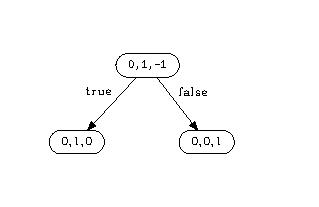
\includegraphics{figure.pdf}
%\vspace*{-0.4in}
\end{center}
\caption{Representation of the $max2$ function}\label{fig:max2}
\end{figure}

\subsection*{Concolic Search}

Overall, \DryadSynth implements the standard CEGIS framework~\cite{sketch}. The verifier is quite straightforward: let the synthesis specification be $\varphi(f, \vec{x})$, then whenever the synthesizer proposes a candidate solution $f_0$, the specification $\forall \vec{x}. \varphi(f_0, \vec{x})$ is encoded as a SMT query and solved by Z3~\cite{Z3}, a state-of-the-art SMT solver. If the verification fails, the counterexample (assignments to $x_1$ through $x_n$) will be added to the accumulated set of counterexamples.

The synthesizer in the CEGIS framework adopts an enumeration strategy: it enumerates all possible heights of the decision tree, starting from $1$. In each iteration of the CEGIS loop, the synthesizer attempts to synthesize a solution with the current height $h$. If there is no solution, the synthesizer increases the height to $h+1$ and retry.

For each synthesis attempt, the height $h$ is fixed and a set of counterexamples $\Gamma$ is available. The synthesis task is to find all field values of the full decision tree of height $h$, representing a function $f_0$, such that for any counterexample $\vec{d}$ in $\Gamma$, the synthesis specification is valid: $\displaystyle \bigwedge_{\vec{d} \in \Gamma} \varphi(f_0, \vec{d})$. 

\DryadSynth symbolically solves the synthesis task by encoding it to a SMT query. Notice that the full decision tree of height $h$ consists of $2^h - 1$ nodes. We first encode the location of each node to a distinct integer between $0$ and $2^h-2$, and represent the field $c_i$ of node $j$ as $c_i^j$. Then each occurrence of $f(\vec{d})$ in the synthesis condition with concrete $\vec{d}$ can be encoded using these field variables. For example, if an assignment $(x_1 = 1, x_2 = 2)$ is a counterexample in $\Gamma$ and the current height is $2$, then the expression $f(1, -2)$ can be represented as a LIA expression $$\textrm{if~} c_0^0 + c_1^0 - 2c_2^0 \geq 0 \textrm{~then~} c_0^1 + c_1^1 - 2c_2^1 \textrm{~else~} c_0^2 + c_1^2 - 2c_2^2$$

\subsection*{Parallelization and Optimization}

While the naive enumeration algorithm incrementally searches all possible height of the decision tree, starting from $1$, the algorithm can be naturally parallelized to leverage the multi-cores, if available. If there are $n$ cores available on the machine, the parallel version \DryadSynth solver runs the same CEGIS algorithm with $n$ different heights on the $n$ cores independently, i.e., each maintains a separate set of counterexamples. The algorithm starts with the $n$ smallest heights, $\{1, \dots, n\}$. It also maintains a variable $p$ as the next height to search, starting from $n+1$. Whenever a core concludes that there is no solution at the current height, it starts a new CEGIS loop at height $p$, and the value of $p$ gets increased. The whole algorithm stops whenever a core finds a solution.

We observed several things from the synthesis results for SyGuS benchmarks:
\begin{enumerate}
\item most of the $c_i$'s are very small. In fact, a lot of benchmarks don't need any coefficient beyond $0$, $1$, or $-1$. 
\item when a benchmark's solution contains large coefficients, there is usually a large coefficient in the specification as well. 
\item if the search space to restricted to solutions with small coefficients only, the performance can be significantly improved. 
\end{enumerate}
These observations allow us to optimize the synthesis algorithm by leveraging a multi-stage strategy. For each height $h$, we split the CEGIS loop into three stages:
\begin{enumerate}
\item in each synthesis iteration, we impose extra constraint $c_i^j \leq 1 \wedge c_i^j \geq -1$ for every $i$ and $j$. Once the synthesis query can't find any solution, move to the next stage --
\item in each synthesis iteration, we impose extra constraint $c_i^j \leq D \wedge c_i^j \geq -D$ where $D$ is a bound such that all coefficients in $\varphi(f, \vec{x})$. Once the synthesis query can't find any solution, move to the next stage --
\item resume the regular synthesis setting, i.e., remove all constraints on coefficients.
\end{enumerate}

We also implemented several simplification strategies. For example, a variable $x$ is irrelevant in an invariant synthesis problem if: a) $x$ does not appear in the $pre$ function or $x'$ does not appear in the $trans$ function; and b) $x$ does not appear in the $post$ function.

%\section{Introduction}
%% no \IEEEPARstart
%This demo file is intended to serve as a ``starter file''
%for IEEE conference papers produced under \LaTeX\ using
%IEEEtran.cls version 1.8b and later.
%% You must have at least 2 lines in the paragraph with the drop letter
%% (should never be an issue)
%I wish you the best of success.
%
%\hfill mds
% 
%\hfill August 26, 2015
%
%\subsection{Subsection Heading Here}
%Subsection text here.
%
%
%\subsubsection{Subsubsection Heading Here}
%Subsubsection text here.


% An example of a floating figure using the graphicx package.
% Note that \label must occur AFTER (or within) \caption.
% For figures, \caption should occur after the \includegraphics.
% Note that IEEEtran v1.7 and later has special internal code that
% is designed to preserve the operation of \label within \caption
% even when the captionsoff option is in effect. However, because
% of issues like this, it may be the safest practice to put all your
% \label just after \caption rather than within \caption{}.
%
% Reminder: the "draftcls" or "draftclsnofoot", not "draft", class
% option should be used if it is desired that the figures are to be
% displayed while in draft mode.
%
%\begin{figure}[!t]
%\centering
%\includegraphics[width=2.5in]{myfigure}
% where an .eps filename suffix will be assumed under latex, 
% and a .pdf suffix will be assumed for pdflatex; or what has been declared
% via \DeclareGraphicsExtensions.
%\caption{Simulation results for the network.}
%\label{fig_sim}
%\end{figure}

% Note that the IEEE typically puts floats only at the top, even when this
% results in a large percentage of a column being occupied by floats.


% An example of a double column floating figure using two subfigures.
% (The subfig.sty package must be loaded for this to work.)
% The subfigure \label commands are set within each subfloat command,
% and the \label for the overall figure must come after \caption.
% \hfil is used as a separator to get equal spacing.
% Watch out that the combined width of all the subfigures on a 
% line do not exceed the text width or a line break will occur.
%
%\begin{figure*}[!t]
%\centering
%\subfloat[Case I]{\includegraphics[width=2.5in]{box}%
%\label{fig_first_case}}
%\hfil
%\subfloat[Case II]{\includegraphics[width=2.5in]{box}%
%\label{fig_second_case}}
%\caption{Simulation results for the network.}
%\label{fig_sim}
%\end{figure*}
%
% Note that often IEEE papers with subfigures do not employ subfigure
% captions (using the optional argument to \subfloat[]), but instead will
% reference/describe all of them (a), (b), etc., within the main caption.
% Be aware that for subfig.sty to generate the (a), (b), etc., subfigure
% labels, the optional argument to \subfloat must be present. If a
% subcaption is not desired, just leave its contents blank,
% e.g., \subfloat[].


% An example of a floating table. Note that, for IEEE style tables, the
% \caption command should come BEFORE the table and, given that table
% captions serve much like titles, are usually capitalized except for words
% such as a, an, and, as, at, but, by, for, in, nor, of, on, or, the, to
% and up, which are usually not capitalized unless they are the first or
% last word of the caption. Table text will default to \footnotesize as
% the IEEE normally uses this smaller font for tables.
% The \label must come after \caption as always.
%
%\begin{table}[!t]
%% increase table row spacing, adjust to taste
%\renewcommand{\arraystretch}{1.3}
% if using array.sty, it might be a good idea to tweak the value of
% \extrarowheight as needed to properly center the text within the cells
%\caption{An Example of a Table}
%\label{table_example}
%\centering
%% Some packages, such as MDW tools, offer better commands for making tables
%% than the plain LaTeX2e tabular which is used here.
%\begin{tabular}{|c||c|}
%\hline
%One & Two\\
%\hline
%Three & Four\\
%\hline
%\end{tabular}
%\end{table}


% Note that the IEEE does not put floats in the very first column
% - or typically anywhere on the first page for that matter. Also,
% in-text middle ("here") positioning is typically not used, but it
% is allowed and encouraged for Computer Society conferences (but
% not Computer Society journals). Most IEEE journals/conferences use
% top floats exclusively. 
% Note that, LaTeX2e, unlike IEEE journals/conferences, places
% footnotes above bottom floats. This can be corrected via the
% \fnbelowfloat command of the stfloats package.




%\section{Conclusion}
%The conclusion goes here.




% conference papers do not normally have an appendix


% use section* for acknowledgment
%\section*{Acknowledgment}
%
%
%The authors would like to thank...





% trigger a \newpage just before the given reference
% number - used to balance the columns on the last page
% adjust value as needed - may need to be readjusted if
% the document is modified later
%\IEEEtriggeratref{8}
% The "triggered" command can be changed if desired:
%\IEEEtriggercmd{\enlargethispage{-5in}}

% references section

% can use a bibliography generated by BibTeX as a .bbl file
% BibTeX documentation can be easily obtained at:
% http://mirror.ctan.org/biblio/bibtex/contrib/doc/
% The IEEEtran BibTeX style support page is at:
% http://www.michaelshell.org/tex/ieeetran/bibtex/
%\bibliographystyle{IEEEtran}
% argument is your BibTeX string definitions and bibliography database(s)
%\bibliography{IEEEabrv,../bib/paper}
%
% <OR> manually copy in the resultant .bbl file
% set second argument of \begin to the number of references
% (used to reserve space for the reference number labels box)
%\begin{thebibliography}{1}
%
%\bibitem{IEEEhowto:kopka}
%H.~Kopka and P.~W. Daly, \emph{A Guide to \LaTeX}, 3rd~ed.\hskip 1em plus
%  0.5em minus 0.4em\relax Harlow, England: Addison-Wesley, 1999.
%
%\end{thebibliography}

\bibliographystyle{IEEEtranS}
\bibliography{refs}





% that's all folks
\end{document}


